\section{Additional Experiment Results}
\begin{figure*}[ht]
    \centering
    % 佔位符: 請替換為 Base 模型的泛化結果圖 (多個子圖)
    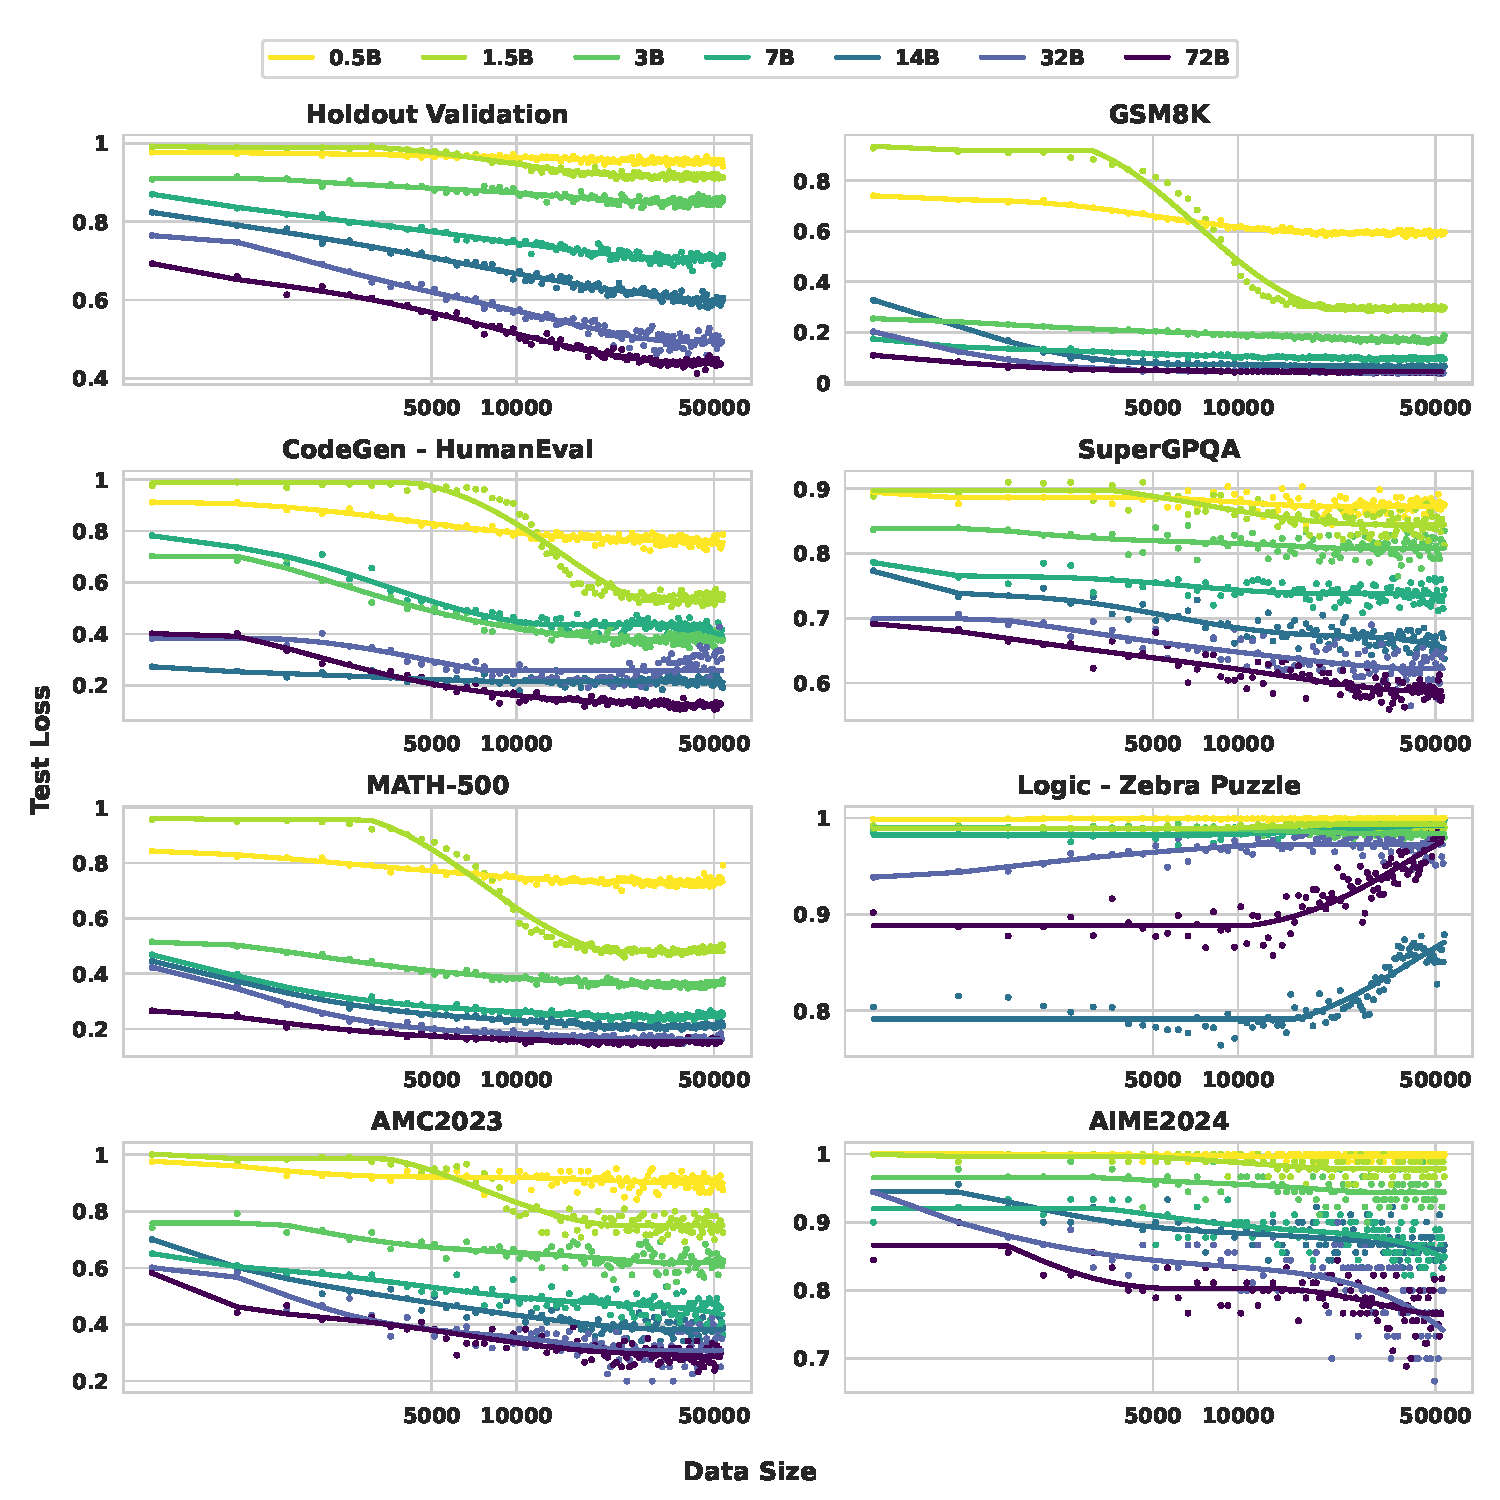
\includegraphics[width=0.7\linewidth]{./figures/allmetric/all_base_E_ErrRate.pdf}
    \caption{Test loss on in-domain and out-of-domain benchmarks vs data size for Base models. It shows modest positive transfer on in-domain tasks, with limited or negative transfer on OOD tasks.}
    \label{fig:generalization_results_base}
\end{figure*}
\label{app:additional_results}

This section provides supplementary experimental results that support and extend the analyses presented in the main body of the paper.

\subsection{Performance on In-Domain and Out-of-Domain Tasks}
\label{app:generalization_tasks}

To assess how the mathematical reasoning capabilities acquired during RL fine-tuning generalize, we evaluated our models on a comprehensive suite of unseen benchmarks. We categorize these into two groups: in-domain different tasks (other mathematics datasets) and out-of-domain tasks (e.g., code, science, logic). The results are presented in Figure~\ref{fig:generalization_results_base} and Figure~\ref{fig:generalization_results_instruct}.




\textbf{In-Domain Generalization (Different Mathematical Tasks).}
On mathematics benchmarks not included in our training set (such as GSM8K, MATH, AIME, and AMC), we observe a generally positive transfer of learned skills. For most of these tasks, the test loss shows a modest but consistent decrease as training progresses, particularly for the larger models. This suggests that the model's enhanced reasoning ability is not overfitted to the training distribution and is applicable to a wider range of mathematical problems.

\textbf{Out-of-Domain Generalization.}
When evaluating on tasks outside of mathematics, the generalization is more limited. For both code generation (HumanEval) and science problems (SuperGPQA), performance remains largely static throughout the training process across all model sizes, with test loss curves staying flat. This indicates that the specialized mathematical reasoning skills do not readily transfer to these domains. A noteworthy phenomenon is observed in the logical reasoning task (Zebra Puzzle): the largest models (particularly the 14B variants) show a degradation in performance (an increase in test loss) as training progresses, suggesting a potential negative transfer effect where intensive optimization on mathematical reasoning may interfere with capabilities required for certain types of logical puzzles.
\begin{figure*}[tb]
    \centering
    % 佔位符: 請替換為 Instruct 模型的泛化結果圖 (多個子圖)
    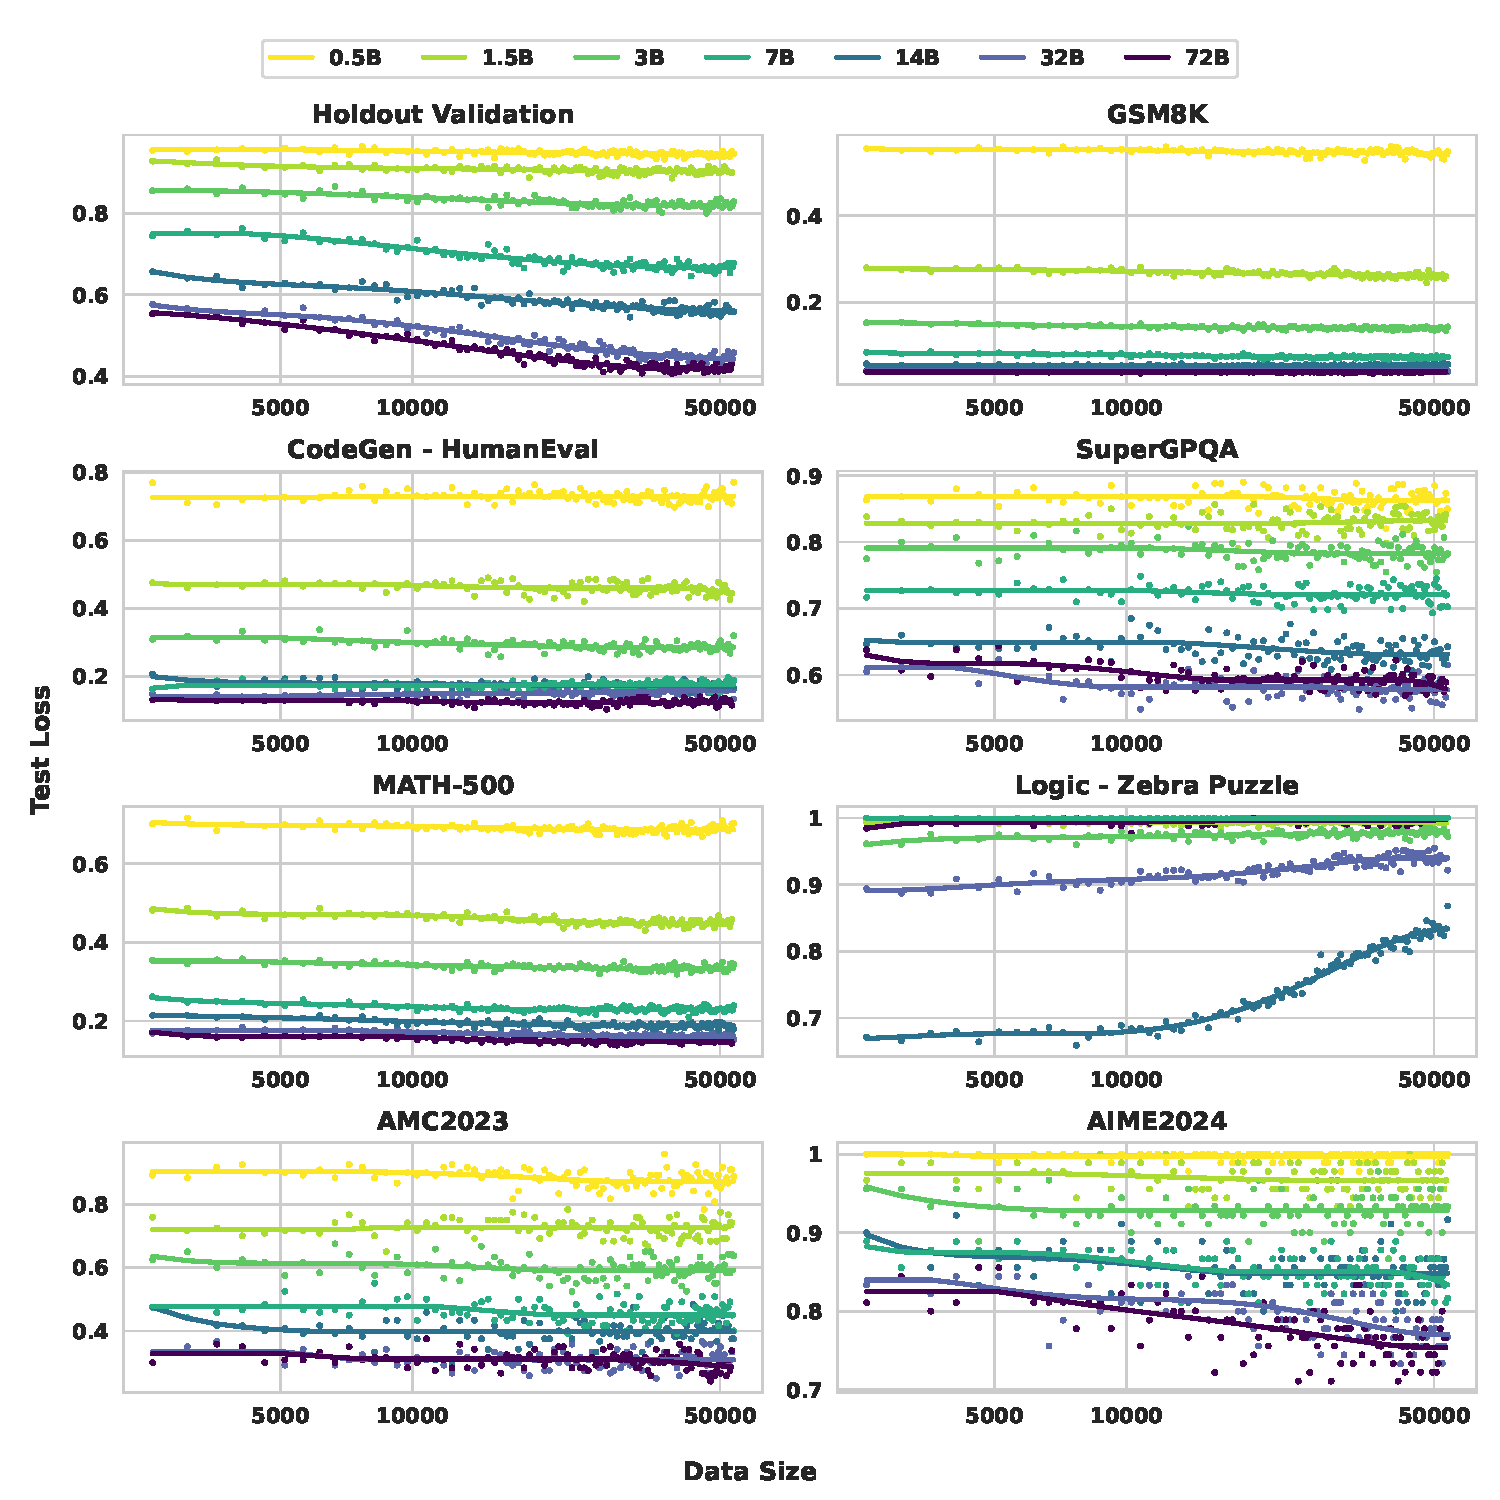
\includegraphics[width=0.7\linewidth]{./figures/allmetric/all_instruct_E_ErrRate.pdf}
    \caption{Test loss on in-domain and out-of-domain benchmarks vs data size for Instruct models.}
    \label{fig:generalization_results_instruct}
\end{figure*}
\subsection{Ablation on GRPO Hyperparameters}
\label{subsec:ablation_grpo}
% \begin{tcolorbox}[colback=blue!5!white, colframe=blue!30!white, title=Observation 6]
% A larger GRPO rollout group size ($G$) is consistently more data-efficient, while the compute-optimal $G$ grows with the total computational budget.
% \end{tcolorbox}
\begin{figure*}[t] % 注意这里改成了 figure*，位置建议用 [t] (top)
    \centering
    
    % --- 第一行 ---
    \begin{subfigure}[t]{0.48\textwidth} % 宽度调整为全页宽的 48%
        \centering
        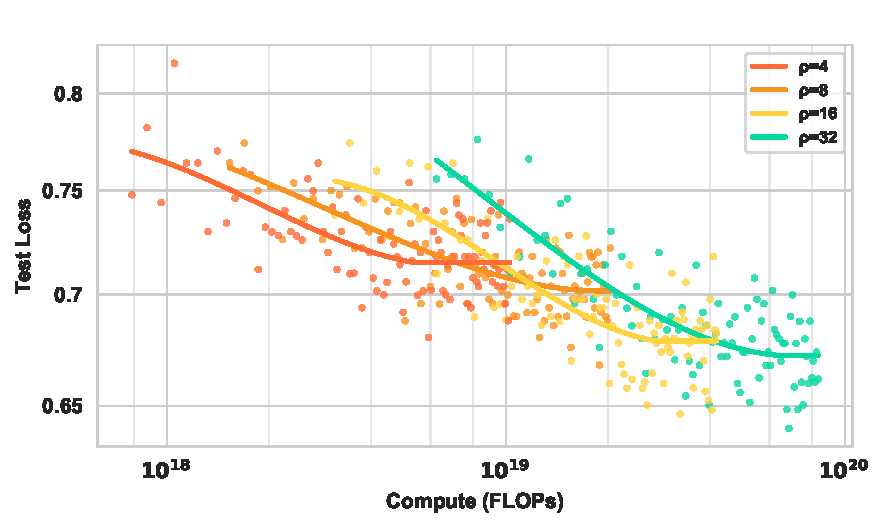
\includegraphics[width=\linewidth]{./figures/grpo/grpo_base_holdout_rollout_n_C_raw_ErrRate.pdf}
        \caption{7B-Base: Loss vs.\ Compute}
        \label{fig:grpo_ablation_a}
    \end{subfigure}
    \hfill % 在两图之间填充空白，使其分别对齐左右边缘
    \begin{subfigure}[t]{0.48\textwidth}
        \centering
        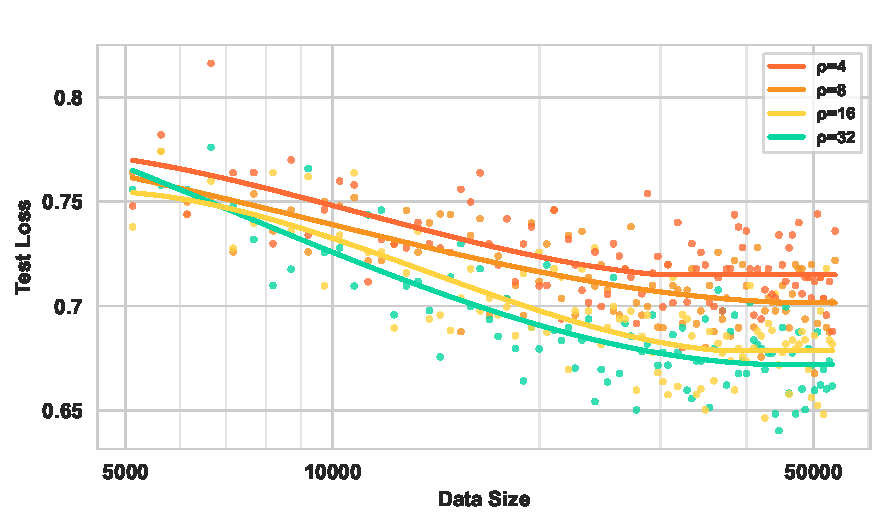
\includegraphics[width=\linewidth]{./figures/grpo/grpo_base_holdout_rollout_n_E_ErrRate.pdf}
        \caption{7B-Base: Loss vs.\ Data Size}
        \label{fig:grpo_ablation_b}
    \end{subfigure}
    
    \vspace{1em} % 增加第一行和第二行之间的垂直间距
    
    % --- 第二行 ---
    \begin{subfigure}[t]{0.48\textwidth}
        \centering
        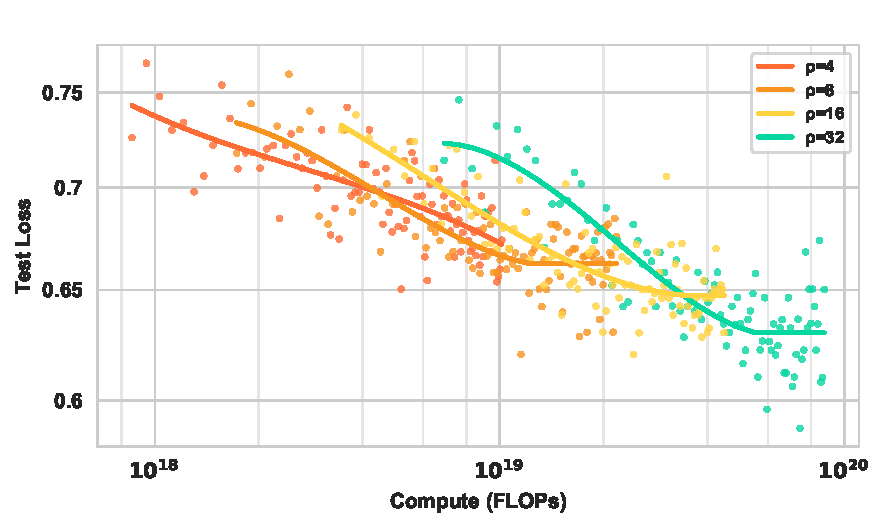
\includegraphics[width=\linewidth]{./figures/grpo/grpo_instruct_holdout_rollout_n_C_raw_ErrRate.pdf}
        \caption{7B-Instruct: Loss vs.\ Compute}
        \label{fig:grpo_ablation_c}
    \end{subfigure}
    \hfill
    \begin{subfigure}[t]{0.48\textwidth}
        \centering
        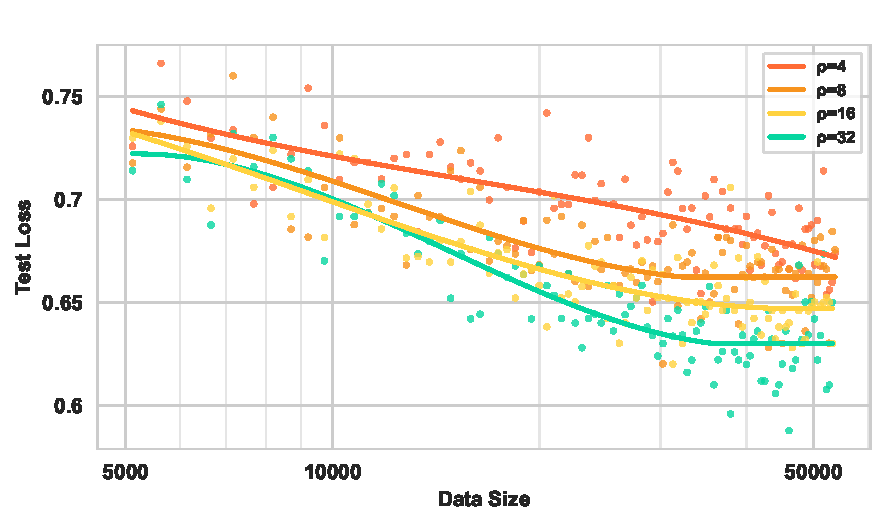
\includegraphics[width=\linewidth]{./figures/grpo/grpo_instruct_holdout_rollout_n_E_ErrRate.pdf}
        \caption{7B-Instruct: Loss vs.\ Data Size}
        \label{fig:grpo_ablation_d}
    \end{subfigure}

    \caption{
        Effects of GRPO rollout size on training efficiency.
        The top row shows the base model results, while the bottom row shows the instruct model results.
    }
    \label{fig:grpo_ablation}
\end{figure*}
We conducted an ablation study on the rollout group size $G$, a key GRPO hyperparameter that controls how many responses are sampled per prompt. This directly affects both the compute per update and the stability of the training signal. We tested $G \in \{4, 8, 16, 32\}$ on the 7B models.

\textbf{Data-centric View}. Figure~\ref{fig:grpo_ablation_b} and \ref{fig:grpo_ablation_d} shows that larger rollout sizes consistently yield better sample efficiency: $G=32$ achieves the lowest test loss for the same number of unique samples. This supports the intuition that more responses per question provide a stronger advantage estimate and thus more effective gradient updates.

\textbf{Compute-centric View}. The optimal rollout size $G$ is not fixed but shifts with the training budget. 
This implies that practitioners should tune $G$ according to available compute rather than relying on a universal setting. 
We attribute this dynamic to the trade-off between the higher variance reduction from larger $G$ and the additional FLOPs it consumes, which makes small $G$ preferable at low budgets but large $G$ superior when ample compute is available.
\subsection{Peformance Compared with Advance Models}
\label{app:sota_comparison}
\begin{figure}[H]
    % --- 左邊的子圖 ---
    \centering
    % 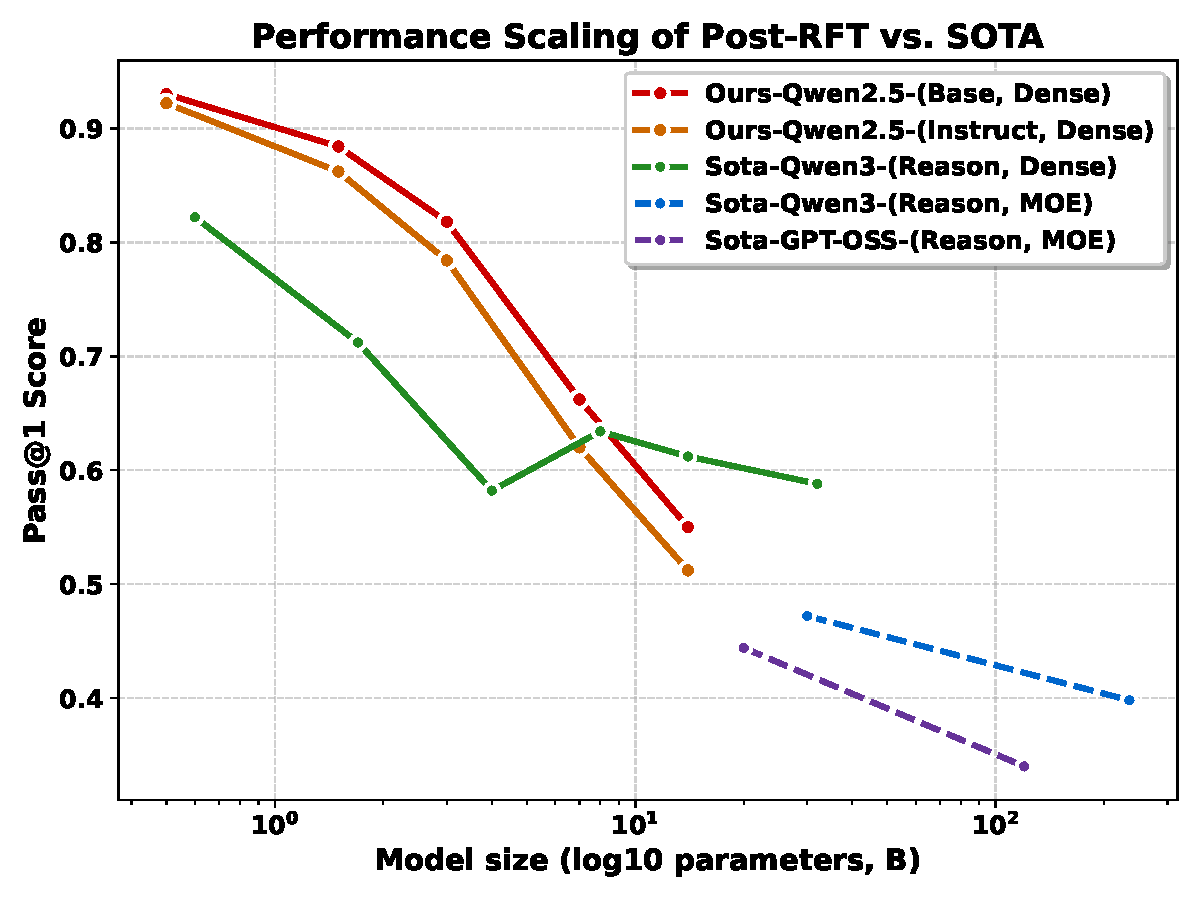
\includegraphics[width=\textwidth]{./figures/plot_scaling.pdf}
    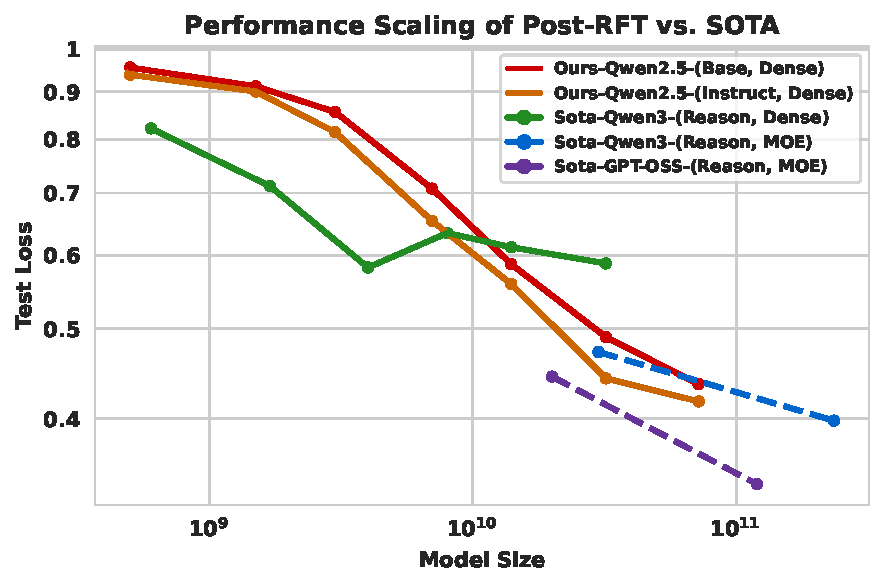
\includegraphics[width=0.9\linewidth]{./figures/outputs/outputs/direct_lines_base_instruct_holdout_E_N_ErrRate.pdf}
    \caption{Relation between test loss and model size $N$ for our trained model and SOTA models demonstrates the effectiveness of our training.}
    \label{fig:loss_vs_model_size}
\end{figure}
We train models of varying sizes to convergence and compare their final test loss. As shown in Figure~\ref{fig:loss_vs_model_size}, larger models consistently achieve lower loss, improving monotonically with scale. The curve shows that smaller models get weaker gains, suggesting diminishing returns at low parameter counts. A likely reason is that larger models inherit richer pre-trained representations, which reinforcement fine-tuning exploits for greater improvements than parameter growth alone. 



We also benchmark our RL-tuned Qwen2.5 models~\citep{qwen2025qwen25technicalreport} against state-of-the-art open-source reasoning systems, including Qwen3~\citep{yang2025qwen3technicalreport} and GPT-OSS~\citep{openai2025gptoss120bgptoss20bmodel}, \tzl{detailed in Table \ref{tab:sota_comparison_appendix}}. \tzl{On our held-out set, the 32B and 72B models match or surpass dense Qwen3 counterparts of similar size, highlighting the effectiveness of RL post-training. Mixture-of-experts models such as Qwen3 and GPT-OSS achieve approximate loss at much larger scales (235B)}, with GPT-OSS-120B currently leading. \tzl{These comparisons suggest that scaling across 0.5B-72B will be necessary to fully characterize post-training behavior and compete with frontier MoE systems.}

\begin{table}[H]
% \begin{wraptable}[12]{r}{0.45\textwidth} 
\centering 
% \resizebox{0.35\columnwidth}{!}{%
\resizebox{0.45\textwidth}{!}{%
\begin{tabular}{llc}
\toprule
\textbf{Model Family} & \textbf{Model Identifier} & \textbf{Pass@1 Score} \\
\midrule
\multicolumn{3}{l}{\textit{Models from Our Study (Post-RFT)}} \\
Qwen2.5-Base & 0.5B & 0.070 \\
             & 1.5B & 0.116 \\
             & 3B   & 0.182 \\
             & 7B   & 0.338 \\
             & 14B  & 0.450 \\
             & \tzl{32B}  & \tzl{0.540} \\
             & \tzl{72B}  & \tzl{0.607} \\
\midrule
Qwen2.5-Instruct & 0.5B & 0.078 \\
                 & 1.5B & 0.138 \\
                 & 3B   & 0.216 \\
                 & 7B   & 0.380 \\
                 & 14B  & 0.488\\
                 & \tzl{32B}  & \tzl{0.590} \\
                 & \tzl{72B}  & \tzl{0.617} \\
\midrule
\multicolumn{3}{l}{\textit{External SOTA Models (for Comparison)}} \\
Qwen3 & 0.6B & 0.178 \\
      & 1.7B & 0.288 \\
      & 4B & 0.418 \\
      & 8B & 0.366 \\
      & 14B & 0.388 \\
      & 30B (A3B) & 0.528 \\
      & 32B & 0.412 \\
      & 235B (A22B) & \textbf{0.602} \\
\midrule
GPT-OSS & 20B  & 0.556 \\
       & 120B  & \textbf{0.660} \\
\bottomrule
\end{tabular}%
}
\caption{Performance of various models on the held-out evaluation set. }
\label{tab:sota_comparison_appendix}
\end{table}
 
To contextualize the performance of our models and the difficulty of our primary evaluation metric, we benchmarked a range of external, state-of-the-art (SOTA) models on our held-out mathematics test set. The results are presented in Table~\ref{tab:sota_comparison_appendix}. The performance of our Qwen2.5 models reflects their final scores after the completion of reinforcement learning fine-tuning (RFT), while others are benchmarked directly.



 



 


 


 



 


 

 
% -------- Figure table begin --------
% \begin{figure*}[t]
%   \centering
%   % -------- Row 1 --------
%   \begin{subfigure}[t]{0.5\textwidth}
%     \centering
%     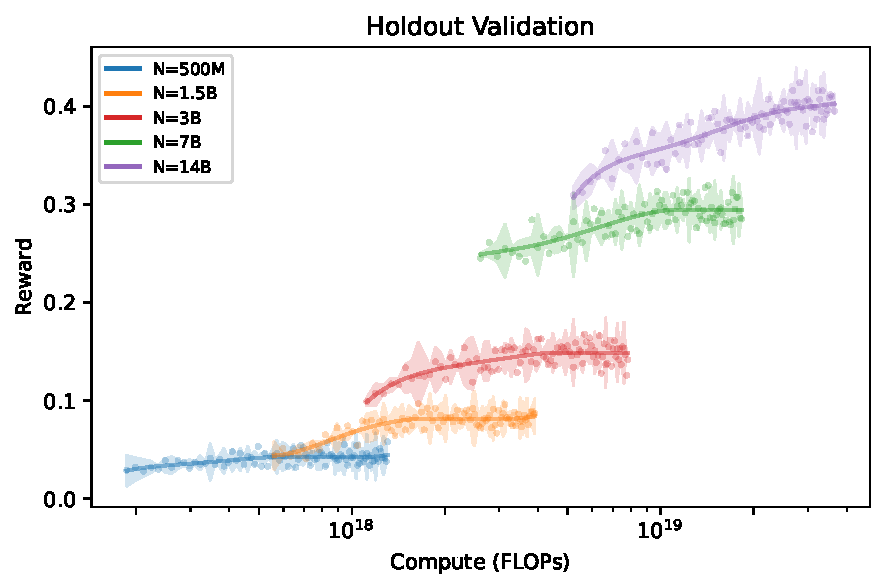
\includegraphics[width=\linewidth]{./figures/holdout/base_holdout_N_C_R.pdf}
%     \label{fig:raw_compute_reward}
%     \caption{Compute (Flops, log) — Reward}
%   \end{subfigure}\hfill
%   \begin{subfigure}[t]{0.5\textwidth}
%     \centering
%     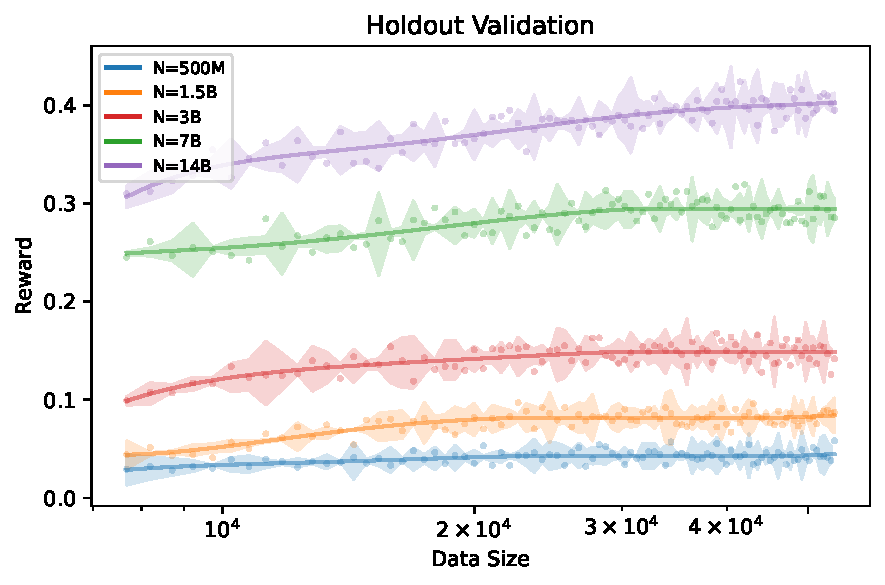
\includegraphics[width=\linewidth]{./figures/holdout/base_holdout_N_E_R.pdf}
%     \caption{Data size (log) — Reward}
%   \end{subfigure}\hfill
%   \par\medskip 
%   % -------- Row 2 --------
%   \begin{subfigure}[t]{0.5\textwidth}
%     \centering
%     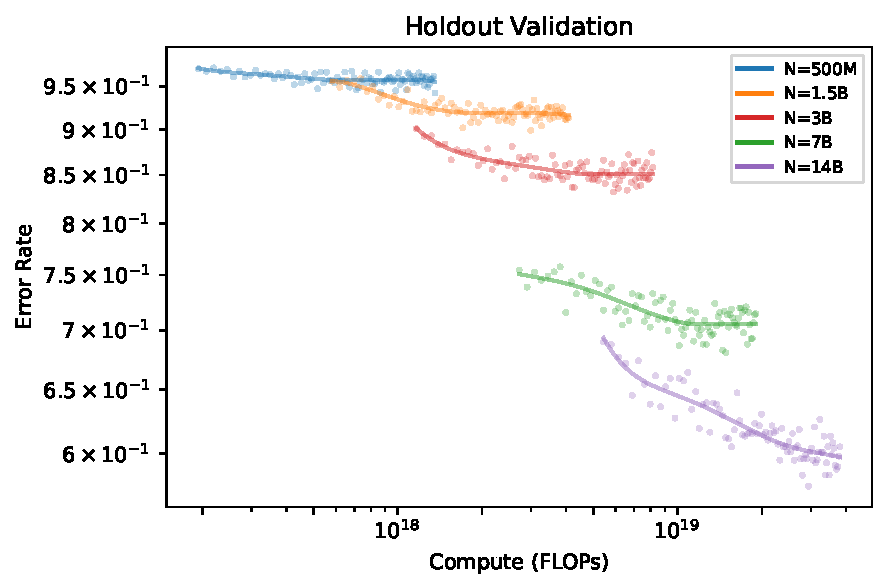
\includegraphics[width=\linewidth]{./figures/holdout/base_holdout_N_C_ErrRate.pdf}
%     \caption{Compute (Flops, log) — error rate}
%   \end{subfigure}\hfill
%   \begin{subfigure}[t]{0.5\textwidth}
%     \centering
%     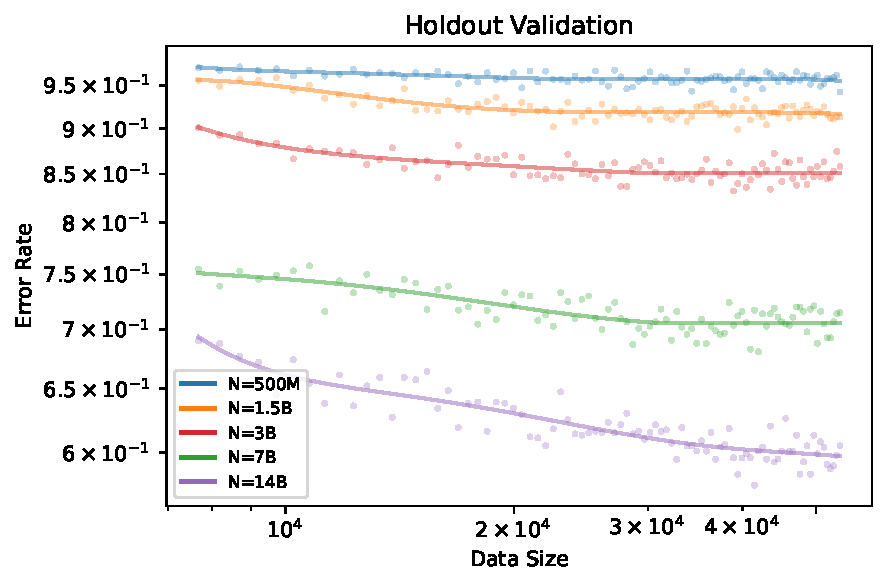
\includegraphics[width=\linewidth]{./figures/holdout/base_holdout_N_E_ErrRate.pdf}
%     \caption{Data size (log) — error rate}
%   \end{subfigure}\hfill

%   \vspace{-0.25em}
%   \caption{Return and Error Rate curves on holdout validation (Base model).}
%   \label{fig:holdout_N_E_C_R_ErrRate_base}
% \end{figure*}





% -------- Figure table begin --------
% \begin{figure*}[t]
%   \centering
%   % -------- Row 1 --------
%   \begin{subfigure}[t]{0.5\textwidth}
%     \centering
%     \includegraphics[width=\linewidth]{./figures/fit/fit_base_holdout_N_C_R.pdf}
%     \label{fig:raw_compute_reward}
%     \caption{Compute (Flops, log) — Reward}
%   \end{subfigure}\hfill
%   \begin{subfigure}[t]{0.5\textwidth}
%     \centering
%     \includegraphics[width=\linewidth]{./figures/fit/fit_base_holdout_N_E_R.pdf}
%     \caption{Data size (log) — Reward}
%   \end{subfigure}\hfill
%   \par\medskip 
%   % -------- Row 2 --------
%   \begin{subfigure}[t]{0.5\textwidth}
%     \centering
%     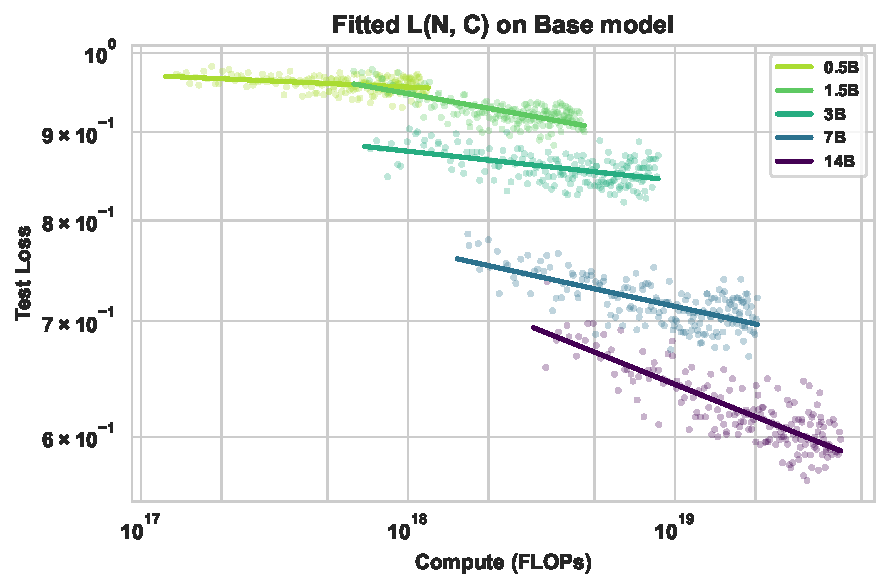
\includegraphics[width=\linewidth]{./figures/fit/fit_base_holdout_N_C_ErrRate.pdf}
%     \caption{Compute (Flops, log) — error rate}
%   \end{subfigure}\hfill
%   \begin{subfigure}[t]{0.5\textwidth}
%     \centering
%     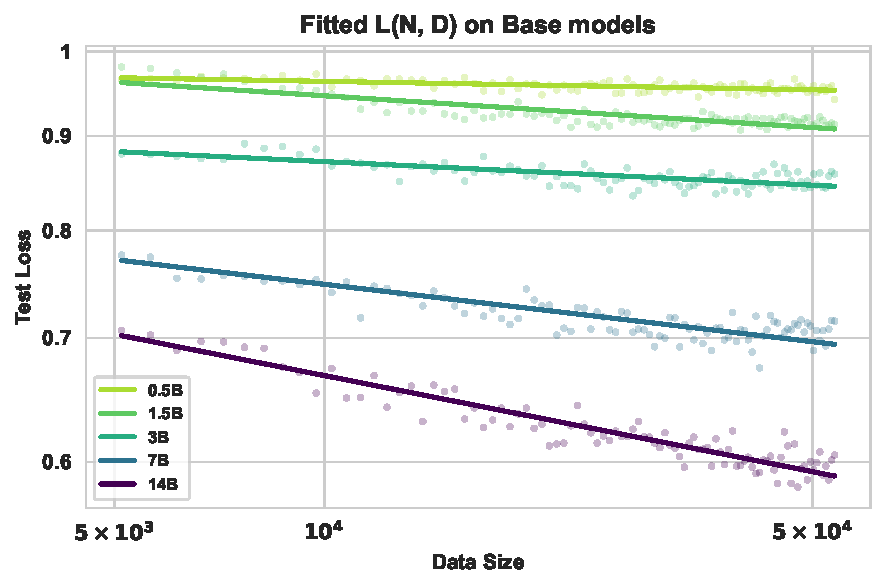
\includegraphics[width=\linewidth]{./figures/fit/fit_base_holdout_N_E_ErrRate.pdf}
%     \caption{Data size (log) — error rate}
%   \end{subfigure}\hfill

%   \vspace{-0.25em}
%   \caption{Fitted curves on holdout validation (Base model).}
%   \label{fig:fit_base_holdout_N_E_C_R_ErrRate}
% \end{figure*}